\documentclass[11pt,a4paper]{article}

%% ===========================================================================
%%  Graph attention in a learned SAT branching heuristic.
%%
%%  Note on GAT-Q-SAT: the attention variant of Graph-Q-SAT, the ablation at
%%  matched training set, and the transfer of the learned heuristic to families
%%  it has never seen.  Engineering (the port, the reproduction oracle, the
%%  restricted heuristics) is confined to section 5, as in the TUDPS and SVM
%%  notes; the instances and the way the numbers are regenerated are in the
%%  appendix.
%% ===========================================================================

\usepackage[T1]{fontenc}
\usepackage[utf8]{inputenc}
\usepackage{amsmath,amssymb}
\usepackage{mathtools}
\usepackage{enumitem}
\usepackage{booktabs}
\usepackage{array}
\usepackage{makecell}
\usepackage{geometry}
\usepackage{placeins}
\usepackage{graphicx}
\usepackage{subcaption}
\usepackage[colorlinks=true,linkcolor=blue,citecolor=blue,urlcolor=blue]{hyperref}
\geometry{margin=2.6cm}
\graphicspath{{img/}}

\newcommand{\code}[1]{\texttt{\def\_{\textunderscore\allowbreak}#1}}
\newcommand{\MRIR}{\mathrm{MRIR}}
\emergencystretch=2em

\title{Attention and transfer in a learned {SAT} branching heuristic:\\
       from Graph-Q-SAT to GAT-Q-SAT}
\author{Donato Meoli\\
        Dipartimento di Informatica, Universit{\`a} di Pisa\\
        Largo B. Pontecorvo 3, 56127 Pisa -- Italy\\
        {\tt donato.meoli@outlook.com}
        }

\date{\today}

\begin{document}
\maketitle

\begin{abstract}
We are concerned with the branching heuristic of a Conflict-Driven Clause
Learning solver for the Boolean satisfiability problem, and with how much of
what such a heuristic learns survives a change of the instances to which it is
applied. Our starting point is Graph-Q-SAT \cite{Kurin2020}, which represents
the state of the search as the bipartite graph of the formula and learns the
action-value function of the corresponding decision process with a graph network
trained by DQN. One set of weights then applies to formulas of any size, so that
the question of transfer can be asked at all. We propose GAT-Q-SAT, a variant in
which the uniform aggregation of the core block is replaced by two edge-aware,
multi-head attention layers, everything else being left as it is, and we measure
the two models along a ladder of test instances that are increasingly far from
the training ones, with attention on and off at matched training set. What the
ladder shows is that the advantage of attention grows with the distance. On the
training distribution it is modest, and it grows with the size of the instances,
from $+0.17$ of median relative iteration reduction on \code{flat30-60} to
$+2.04$ on \code{flat200-479}, where the plain model degrades to $1.35$ while
the attention one holds at $3.39$. Under a change of distribution (trained
on uniform random 3-SAT and tested on graph colouring) the plain model falls
below the heuristic it replaces at every size ($0.78$ to $0.97$) while the
attention one stays above it ($1.16$ to $1.75$). Under a change of domain, i.e.,
taken with no retraining of any kind to four SATLIB families that it has never
seen, the attention model is at or above the reference solver on three of the
four (AIM $1.29$, quasigroup $1.01$, planning $1.14$) and the plain one on one
(AIM $1.50$). What attention buys is therefore not so much a better heuristic on
the instances one trains on, as a heuristic that keeps working on the instances
one does not. The boundary is where there is no structure to be weighted: on
uniform random 3-SAT at the phase transition attention gives nothing, and costs
a factor of three; we also find that this advantage of the plain aggregation is confined to the
satisfiable instances, the ordering being reversed on the unsatisfiable families
of the same generator. Of course, fewer iterations need not be less time, and at
this scale they are not, each decision being a forward pass of the network; we
report the wall-clock cost as measured. The whole study rests on a port of the
original implementation to a current PyTorch stack, whose semantics is checked
by reproducing the published evaluation of the original checkpoints to the last
digit.
\end{abstract}

%% ===========================================================================
\section{Introduction}\label{sec:intro}
%% ===========================================================================

We are concerned with the branching heuristic of a solver for the Boolean
satisfiability problem (SAT), i.e., with the rule that decides which
variable the search assigns next, and with the question of whether such a rule
can be learned from data instead of being hand-crafted. The solvers we consider
implement the Conflict-Driven Clause Learning scheme (CDCL), in which the search
repeatedly (i) decides a variable and assigns a value to it, (ii) propagates the
assignments that become implied, and (iii) upon a conflict, learns a clause and
backjumps to the level that the clause allows \cite{EenSorensson2003}. The choice
at point (i) is delegated to a heuristic, in practice some variant of VSIDS,
which ranks the variables by counters updated at each conflict. Those counters
carry no information at the beginning of the search, and they are in any case a
rough surrogate of the quantity one would really want, that is, the variable
whose assignment prunes the largest subtree. The heuristic is therefore a
natural place where a learned policy can be inserted, and a convenient one,
since a bad decision costs time but never correctness: whatever the policy does,
the solver remains sound and complete.

\smallskip
\noindent
The literature on learning for SAT can be organised according to what the
network is asked to produce, and to when it is queried. NeuroSAT
\cite{Selsam2019} learns satisfiability itself from single-bit supervision,
showing that message passing \cite{Gilmer2017} captures something of the
structure of a formula; NeuroCore \cite{SelsamBjorner2019} moves to a quantity
that a solver can consume, the variables that occur in an unsatisfiable core,
and uses the prediction to re-rank the VSIDS activities periodically. NeuroComb
and NeuroBack \cite{Wang2024} query the network only once, before the solve, so
that inference is paid offline and wall-clock gains on industrial instances
become possible. Along a different line, the branching policy is learned by
reinforcement rather than by supervision: Graph-Q-SAT \cite{Kurin2020}
represents the state as the bipartite graph of the formula, and learns the
action-value function of the corresponding decision process with DQN
\cite{Mnih2015}. One set of weights then applies to formulas of any size, the
network reading a graph rather than a fixed-size encoding of one. It is on this
that we build, and for a precise reason: a heuristic of that kind is the only
one to which the question we are interested in can be put at all, which is what
it does on instances that do not look like the ones it was trained on.

\smallskip
\noindent
What we do is the following. First, we propose GAT-Q-SAT, a variant of
Graph-Q-SAT in which the uniform aggregation over the neighbours of a node is
replaced by two edge-aware, multi-head attention layers \cite{Velickovic2018}
inside the core block, the rest of the architecture being left as it is. The
learned weighting can only pay where the neighbourhood is not homogeneous, and
the point of the experiments is to establish where that is. Second, we measure the two
models in the ablation that the available runs make possible, attention on and
off at matched training set, along a ladder of test instances that are
increasingly far from the training ones: the training distribution itself, then
the larger instances of the same family, then a different distribution, and
finally four families that the models have never seen, on which the
colouring-trained weights are used with no retraining and no fine-tuning of any
kind. Third, we read the ladder rather than its single rungs, since that is
where the result is. That attention helps in distribution is a matter of a few
tenths of MRIR where the test instances resemble the training ones; what the
ladder adds is that the help grows with the distance, to the point where the
plain model falls below the heuristic it is meant to replace exactly in the
regimes in which the attention one keeps working. Underneath all of this there is an engineering step without which none
of the three could be checked. The original implementation rests on a software
stack that can no longer be installed as it stands, so we port it to a current
one, using the reproduction of the published evaluation of the original
checkpoints as the test that the port has not changed the semantics.

\smallskip
\noindent
The structure of this note is the following. \S~\ref{sec:problem} recalls the
decision process that the branching problem defines and the value-based
algorithm that solves it. \S~\ref{sec:gqsat} describes Graph-Q-SAT, that is, the
graph representation of the state and the encode--process--decode network that
scores the actions, and \S~\ref{sec:gat} the attention variant that we propose,
together with what it costs. \S~\ref{sec:impl} is devoted to the implementation:
the port, the reproduction used as a non-regression oracle, and the restricted
heuristics that we have added at evaluation time. \S~\ref{sec:results} reports the
computational results, and it is organised as the ladder itself: the training
distribution (\S~\ref{sec:indist}), a change of size, a change of distribution
(\S~\ref{sec:shift}) and a change of domain (\S~\ref{sec:transfer}), followed by
the regime in which attention does not help and by what a change of
satisfiability does there (\S~\ref{sec:boundary}), and by the wall-clock cost of
a decision (\S~\ref{sec:time}). \S~\ref{sec:conc} draws the
conclusions, and Appendix~\ref{app:instances} describes the instances and the
way in which every number of \S~\ref{sec:results} is regenerated.

\smallskip
\noindent
Throughout the note the following notation is used. A formula in conjunctive
normal form has $n$ variables and $m$ clauses; a decision is the assignment of a
truth value to an unassigned variable. The quality of a heuristic is measured,
as in \cite{Kurin2020}, by the Median Relative Iteration Reduction: for each
instance one takes the number of iterations of the reference solver divided by
the number of iterations of the model, and then the median over the instances of
a set,
\begin{equation}\label{eq:mrir}
  \MRIR = \operatorname{median}\,
          \frac{\#\text{iterations of MiniSat}}{\#\text{iterations of the model}} \, ,
\end{equation}
so that a value larger than $1$ means fewer iterations than the baseline and $1$
means parity. Every evaluation is run with a cap on the number of decisions that
the model is allowed to take, after which control returns to VSIDS for the rest
of the solve; ``cap $k$'' denotes the evaluation with that cap set to $k$.
Instance families keep their SATLIB \cite{HoosStutzle2000} names.
\code{uf}$n$-$m$ and \code{uuf}$n$-$m$ are satisfiable and unsatisfiable uniform
random 3-SAT with $n$ variables and $m$ clauses, while \code{flat}$n$-$m$ are
the graph-colouring ones.

%% ===========================================================================
\section{Branching as a decision process}\label{sec:problem}
%% ===========================================================================

The solver is the environment of a Markov Decision Process, whose state is the
formula together with the current partial assignment, whose actions are the
admissible branching decisions, and whose dynamics are the solver itself: a step
is one decision followed by all the propagation and the backjumping that the
decision triggers, so that the transition is deterministic but known only by
running it. The reward is a constant $-p$ at each non-terminal step and $0$ at
termination, hence maximising the return means terminating in as few decisions
as possible, which is the quantity that \eqref{eq:mrir} measures.

\smallskip
\noindent
The policy is learned by DQN \cite{Mnih2015}: the optimal action-value function
\begin{equation}\label{eq:bellman}
  Q^\star(s,a) = \mathbb{E}\big[\,r + \gamma \max_{a'} Q^\star(s',a')\,\big]
\end{equation}
is approximated by a network $Q_\theta$ fitted on the temporal-difference error
over a replay buffer, with a target network $\theta^-$ providing the bootstrap
and an $\varepsilon$-greedy behaviour policy providing the exploration; the
heuristic is then $\pi(s) = \arg\max_a Q_\theta(s,a)$. Two features of the
problem constrain the approximator, and it is worth stating them before the
architecture is described. The action set is variable, since there is one action
per unassigned variable, and it shrinks along an episode; and the state is a
formula, an object defined up to a permutation of its variables and of its
clauses. The network must therefore score a variable number of actions and be
invariant under those permutations, which rules out the fixed-size architectures
and leads to the graph representation of the next section.

%% ===========================================================================
\section{Graph-Q-SAT}\label{sec:gqsat}
%% ===========================================================================

The state is represented \cite{Kurin2020} as the bipartite graph whose nodes are
the variables and the clauses that are still in play, with an edge between a
variable and each clause in which it occurs; the node features are
2-dimensional one-hot vectors distinguishing the two kinds of node, the edge
features encode the polarity of the literal, and the global attribute is empty.
There are two actions per unassigned variable (assign it true, or false), and
the agent takes the $\arg\max$ of the $Q$-values that the network produces on
the variable nodes.

\smallskip
\noindent
The approximator is an encode--process--decode graph network
\cite{Battaglia2018}: an encoder applies one independent block to the edges, the
nodes and the global attribute; the core block, whose weights are shared, is
applied $M$ times, each application updating first the edges, then the nodes,
then the global attribute,
\begin{equation}\label{eq:gnblock}
  e_k' = \phi^e\big(e_k, v_{r_k}, v_{s_k}, u\big) \, , \quad
  v_i' = \phi^v\big(\rho^{e\to v}(\{e_k'\}), v_i, u\big) \, , \quad
  u'   = \phi^u\big(\rho^{e\to u}(\{e_k'\}), \rho^{v\to u}(\{v_i'\}), u\big) \, ,
\end{equation}
with $\phi$ multi-layer perceptrons and $\rho$ permutation-invariant
aggregations, the sum in the original design. A decoder then reads the
$Q$-values off the variable nodes; Figure~\ref{fig:epd} gives the three blocks
and the way they are composed. Since the weights are shared across the nodes and
across the $M$ rounds, one set of them applies to a formula with any number of
variables and clauses, and $M$ can be changed at test time without retraining,
which the implementation exposes as a parameter of the evaluation.

\begin{figure}[h]
\centering
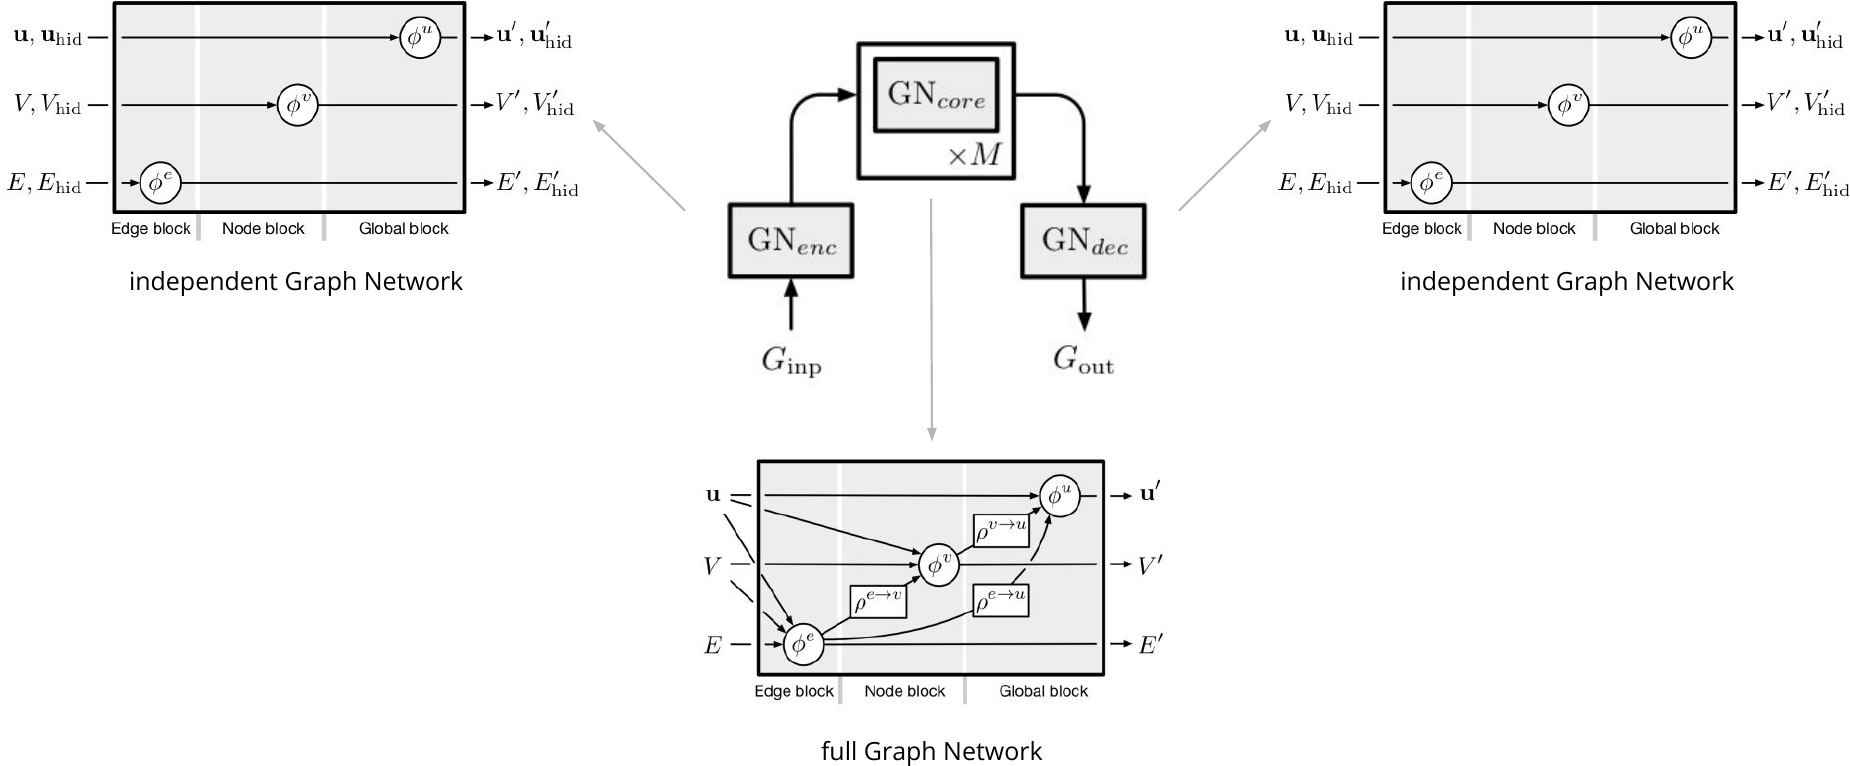
\includegraphics[width=0.86\textwidth]{gqsat_epd.png}
\caption{The encode--process--decode architecture of Graph-Q-SAT: an independent
block encodes the edges, the nodes and the global attribute, a full graph-network
block is applied $M$ times with shared weights, and a second independent block
decodes the $Q$-values. Blocks drawn after \cite{Battaglia2018}.}
\label{fig:epd}
\end{figure}

\smallskip
\noindent
The aggregation $\rho^{e\to v}$ in \eqref{eq:gnblock} is where the model commits
itself: summing the incoming messages says that all the clauses in which a
variable occurs are equally informative about how good it is to branch on it.
For a formula drawn uniformly at random this is not a bad assumption, all the
clauses being statistically alike; for a formula that encodes something, it is
one that throws away exactly the structure that the encoding put there.

%% ===========================================================================
\section{GAT-Q-SAT}\label{sec:gat}
%% ===========================================================================

We replace the uniform aggregation of the core block with the attention of
\cite{Velickovic2018}: the neighbours of a node are weighted by a
coefficient that is itself learned. With a shared linear map $W$, a node $i$ and
its neighbourhood $\mathcal N_i$,
\begin{equation}\label{eq:gat}
\begin{aligned}
  s_{ij} &= \mathrm{LeakyReLU}\big(\mathbf a^{\!\top}
            [\,W h_i \,\|\, W h_j \,\|\, W_e e_{ij}\,]\big) \, ,
  \qquad
  \alpha_{ij} = \operatorname{softmax}_j\big(s_{ij}\big) \, , \\[1mm]
  h_i' &= \sigma\Big(\textstyle\sum_{j\in\mathcal N_i} \alpha_{ij}\, W h_j\Big) \, ,
\end{aligned}
\end{equation}
where $e_{ij}$ is the feature of the edge (the polarity of the literal),
which enters the score $s_{ij}$ through $W_e$ and makes the attention
edge-featured; $K$ independent heads are computed and concatenated.
Two such layers are inserted in the core block, so that the node embeddings are
refined by attention before the global attribute is updated; in the language of
\cite{Battaglia2018} the core stops being a full graph-network block and becomes
a \emph{non-local} one, which is the substitution drawn in
Figure~\ref{fig:gatepd}. Everything else (the encoder, the decoder, the number
of core steps, the reward, the replay buffer and the training schedule) is left
exactly as in \S~\ref{sec:gqsat}, which is what makes the comparison of
\S~\ref{sec:results} an ablation of the aggregation alone.

\begin{figure}[h]
\centering
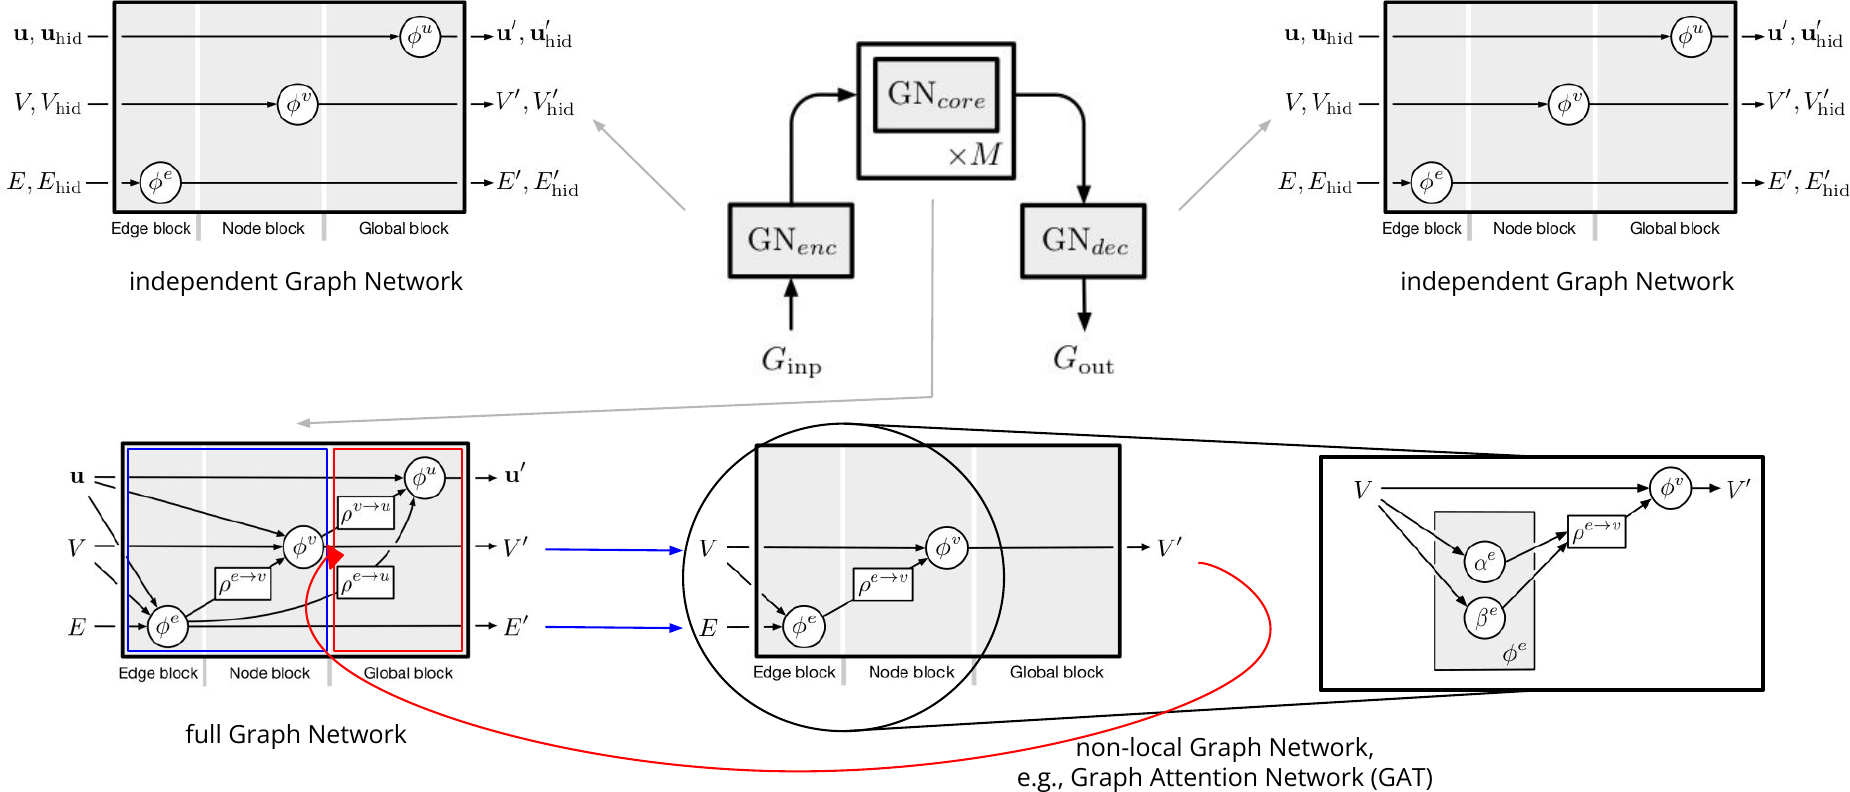
\includegraphics[width=\textwidth]{gatqsat_epd.png}
\caption{GAT-Q-SAT: the core block of Figure~\ref{fig:epd} is replaced by a
non-local one, in which the edge function computes the attention coefficients
$\alpha^e$ and $\beta^e$ of \eqref{eq:gat} and the node function aggregates the
messages weighted by them. Blocks drawn after \cite{Battaglia2018}.}
\label{fig:gatepd}
\end{figure}

\smallskip
\noindent
What one expects from this is bounded, and it is worth saying in advance. The
attention coefficients can only carry information where the neighbours of a node
differ in a way that matters for the decision, that is, where the instance has a
sub-structure that the encoding has left in the graph. On a uniform random
formula at the phase transition there is no such thing, and the layers can only
add parameters to fit and cost per decision to pay. We remark that the cost is
real: the attention is computed on every edge at every core step, so a decision
of GAT-Q-SAT is appreciably more expensive than a decision of Graph-Q-SAT, and
\S~\ref{sec:time} measures how much.

%% ===========================================================================
\section{Implementation}\label{sec:impl}
%% ===========================================================================

The original implementation of \cite{Kurin2020} is built on TensorFlow~1.x for
the network and on a patched MiniSat \cite{EenSorensson2003}, exposed to Python
as a gym environment through a SWIG wrapper, for the solver; the graph part
rests on pinned versions of \code{torch-scatter} and \code{torch-sparse}, which
have to be compiled against the exact version of torch and are the single most
frequent cause of a failed installation. The stack cannot be installed as it
stands today, so the first step is a port, and the difficulty of a port of this
kind is not that it runs, but that it computes the same thing.

\smallskip
\noindent
{\bf The port.} We move the model to the current torch and PyTorch-Geometric
\cite{FeyLenssen2019}. The scattered aggregations of \eqref{eq:gnblock} are
taken from \code{torch\_geometric.utils.scatter}, which removes the two compiled
dependencies altogether. The environment is constructed directly instead of
going through \code{gym.make}, whose checker rejects the non-standard signatures
\code{step(decision, dummy)} and \code{reset(max\_decisions\_cap)} that the
MiniSat wrapper uses, so that the same code runs on the old gym and on
\code{gymnasium}. A loader reconciles the naming of the attention parameters
across PyTorch-Geometric versions (\code{lin\_src} and \code{lin\_dst} against
\code{lin}), which is what allows a checkpoint trained in 2021 to be read today;
the two halves are verified to be equal before they are merged, so the
remapping is lossless. The SWIG wrapper of the solver is regenerated and rebuilt
against \code{numpy}~$\geq 2$.

\smallskip
\noindent
{\bf The reproduction oracle.} That a port of this size has not changed the
semantics is not something one establishes by inspection. We establish it by
re-running the evaluation of the original trained checkpoints on the new stack
and comparing with the logs committed with them: the numbers coincide, e.g., on
\code{flat30-60} at cap $500$ the median MRIR is $1.833$ for Graph-Q-SAT and
$1.667$ for GAT-Q-SAT, as in the originals. Inference exercises the
representation, the message passing, the decoder and the environment stepping at
once, so this is a reasonably strong test, and it is the one we have run after
each step of the port. It says nothing about the training path, which is
exercised separately by retraining both variants from scratch. The configuration
of the published runs is fixed in the training script, since a few default
values of the command line (the cap on the decisions during training first of
all) are enough to make a run converge to something quite different.

\smallskip
\noindent
{\bf Restricted heuristics.} Since the cost of the model is paid at every
decision (cf. \S~\ref{sec:time}), the evaluation loop also implements the three
devices of \cite{Shirokikh2023}, which trade decisions of the model for time. In the \emph{early release} the
model guides the first $N$ decisions, and control then returns to VSIDS for
good; in the \emph{action pool} one forward pass produces the $K$ best actions,
which are executed without querying the network again; in the \emph{warm start}
the $Q$-values at the root are written into the activity counters of the solver,
which then runs pure VSIDS. The last one needs the solver to be told, which the C++ side did not
allow: we have added a method that writes the activities and rebuilds the order
heap, and exposed it through the wrapper. These devices are machinery that the
implementation offers, and we do not report measurements of them here. On the
small instances of \S~\ref{sec:results} they can only lose, their point being
the wall-clock behaviour on instances large enough for the solve to dominate the
inference.

%% ===========================================================================
\section{Computational results}\label{sec:results}
%% ===========================================================================

The instances are those of SATLIB \cite{HoosStutzle2000} described in
Appendix~\ref{app:instances}: uniform random 3-SAT with 50, 100 and 250
variables, satisfiable and unsatisfiable, and graph colouring from 30 to 200
nodes. The runs that are available pair attention on and off at matched training set.
One run per variant is trained on graph colouring (\code{flat50-115}); two runs
per variant are trained on satisfiable uniform random 3-SAT (\code{uf50-218} and
\code{uf100-430}), and their results are averaged over the two; four further runs,
two per variant, are trained on unsatisfiable random formulas and are used only in
\S~\ref{sec:boundary}, where they serve as a control. This is what makes the comparison an ablation of
\eqref{eq:gat} rather than a comparison of two training histories. We report the
MRIR at cap $500$ unless otherwise stated. The evaluations are run on a single
core of a CPU, the networks being small enough that a GPU brings no measurable
advantage at inference, and the environment being a sequential C++ solver behind
a wrapper in any case. The training runs that we re-executed to validate the
training path were done on the T4 GPU of a Colab instance.

\smallskip
\noindent
{\bf What the clock includes.} The times of \S~\ref{sec:time} are taken per
instance around the whole episode, hence they include the parsing of the file,
the construction of the graph and every forward pass of the network. They
exclude the loading of the checkpoint, the construction of the environment, and
the reference run of the solver, whose iteration counts are computed once per
data set and stored as metadata; the ratios of \eqref{eq:mrir}, on the other
hand, are counts of iterations and are therefore unaffected by any of this. Two
figures from different regimes are not to be compared on the absolute value of
the time, the instances of the regimes being of different sizes.

\smallskip
\noindent
{\bf The ladder.} What we measure is one quantity, \eqref{eq:mrir}, on test
instances that stand at four increasing distances from the ones the models were
trained on. The first is no distance at all: train on graph colouring and test
on graph colouring (\S~\ref{sec:indist}). The second is a change of the size of
the instances, the training family being \code{flat50-115} and the test families
going up to \code{flat200-479}, which is the same rung read across the sizes.
The third is a change of the distribution, with models trained on uniform
random 3-SAT and tested on colouring (\S~\ref{sec:shift}). The fourth is a
change of the domain, the colouring-trained weights being applied, with nothing
retrained and nothing tuned, to four families of a different nature
(\S~\ref{sec:transfer}). Everything else is held fixed along the ladder: the
same two checkpoints per rung, the same cap, the same reference solver, and the
same metric. \S~\ref{sec:boundary} then reports the one regime in which attention does not
help at all, together with a fifth rung that the same models give for free,
i.e., a change of satisfiability, and \S~\ref{sec:time} says what a decision
costs in seconds rather than in iterations.

\smallskip
\noindent
{\bf Correctness, before any of it.} The models of the two variants are the ones
released with \cite{Kurin2020}, re-evaluated on the ported stack of
\S~\ref{sec:impl}, and they reproduce the published numbers exactly, e.g.,
$1.833$ and $1.667$ of median MRIR on \code{flat30-60} at cap $500$. The two
models therefore differ by the aggregation of \eqref{eq:gat} and by nothing
else, which is what the rest of this section rests on.

\subsection{On the training distribution}\label{sec:indist}

Trained and tested on graph colouring, GAT-Q-SAT is better than Graph-Q-SAT at
every size, and the difference grows with the size, as Table~\ref{tab:numbers}
shows. The first column is the SATLIB family, whose name gives the number of
nodes and of edges of the underlying graph. The second and the third are the
mean MRIR at cap $500$ of the plain and of the attention model, each averaged
over the runs of the corresponding group, and $\Delta$ is their difference,
positive when attention is the better of the two.

\begin{table}[h]\centering\small
\begin{tabular}{lccc}
\toprule
graph-colouring set & Graph-Q-SAT & GAT-Q-SAT & $\Delta$ \\
\midrule
\code{flat30-60}   & 1.83 & 2.00 & $+0.17$ \\
\code{flat75-180}  & 2.37 & 2.94 & $+0.58$ \\
\code{flat125-301} & 2.55 & 3.44 & $+0.88$ \\
\code{flat150-360} & 1.92 & 3.76 & $+1.85$ \\
\code{flat200-479} & 1.35 & 3.39 & $+2.04$ \\
\bottomrule
\end{tabular}
\caption{In-distribution graph colouring, mean MRIR at cap $500$; the advantage
of attention grows with the size of the instances.}
\label{tab:numbers}
\end{table}

\noindent
On the family closest to the training one the two models are within $0.17$ of
each other, which is the honest measure of what attention is worth when the test
instances look like the training ones. The interesting quantity is how that
number behaves as the instances grow: the plain model degrades, from $2.55$ on
\code{flat125-301} to $1.35$ on \code{flat200-479}, while the attention one does
not, so that the gap becomes $+2.04$. The two are trained on the same family of
50 nodes, hence the largest test instances are already four times the training
size, and this rung of the ladder is a transfer across the size: what the table
says is that the plain aggregation degrades under it and the attention one
holds. Figure~\ref{fig:flatpair} gives the same comparison family by family and as a
function of the decision budget, so that the reading depends neither on the cap
nor on the average over the families. The two panels share the vertical scale.
Graph-Q-SAT peaks at ten decisions and then decays as it is allowed to decide
more, until on \code{flat175-417} and \code{flat200-479} it ends below $1$,
so that the more the plain model decides the worse it does; GAT-Q-SAT rises to
between $1.8$ and $2.4$ and stays there at every budget and on every family.
This is the same statement as the $\Delta$ column of Table~\ref{tab:numbers},
read on eight curves instead of five numbers.

\begin{figure}[h]
\centering
\begin{subfigure}{0.49\textwidth}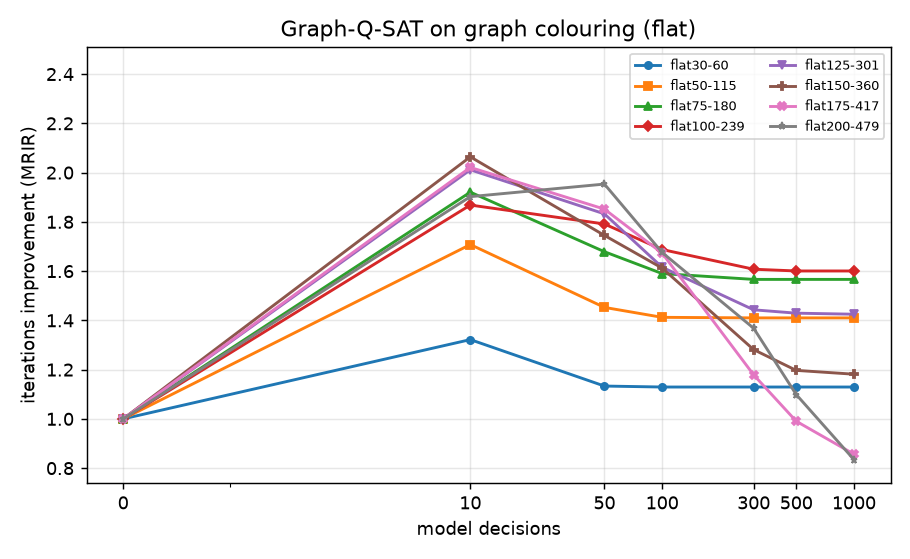
\includegraphics[width=\textwidth]{graphqsat.png}\end{subfigure}
\hfill
\begin{subfigure}{0.49\textwidth}
\includegraphics[width=\textwidth]{gatqsat.png}\end{subfigure}
\caption{MRIR against the decision budget on the eight graph-colouring families,
for the plain model (left) and for the attention one (right), on a common
vertical scale. The plain model decays with the budget and two families fall
below the reference solver; the attention one does not.}
\label{fig:flatpair}
\end{figure}

\subsection{A change of distribution}\label{sec:shift}

The next rung changes what the models were trained on. Both are trained on
satisfiable uniform random 3-SAT, which has nothing of the structure of a
coloured graph, and are evaluated on the colouring families. Graph-Q-SAT falls below $1$ at
every size (between $0.78$ and $0.97$), i.e., it does worse than the heuristic
it replaces, whereas GAT-Q-SAT stays above it (between $1.16$ and $1.75$): the
distinction here is not between a larger and a smaller gain, but between a
heuristic that is worth using and one that is not.
Figure~\ref{fig:thesis} puts the three regimes side by side at cap $500$, and
Figure~\ref{fig:transfercurve} gives this one against the decision budget.

\begin{figure}[h]
\centering
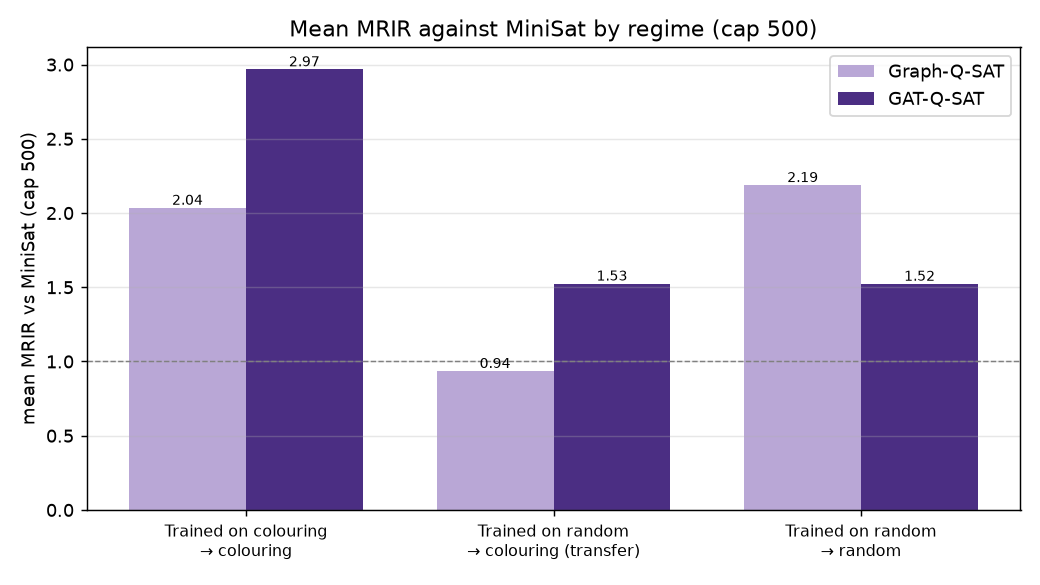
\includegraphics[width=0.78\textwidth]{thesis.png}
\caption{Mean MRIR against MiniSat (cap $500$) per regime: trained and tested on
colouring, trained on random and tested on colouring, trained and tested on
random. Attention helps in the first two, and the gap widens where the training
and the test instances differ.}
\label{fig:thesis}
\end{figure}

\begin{figure}[h]
\centering
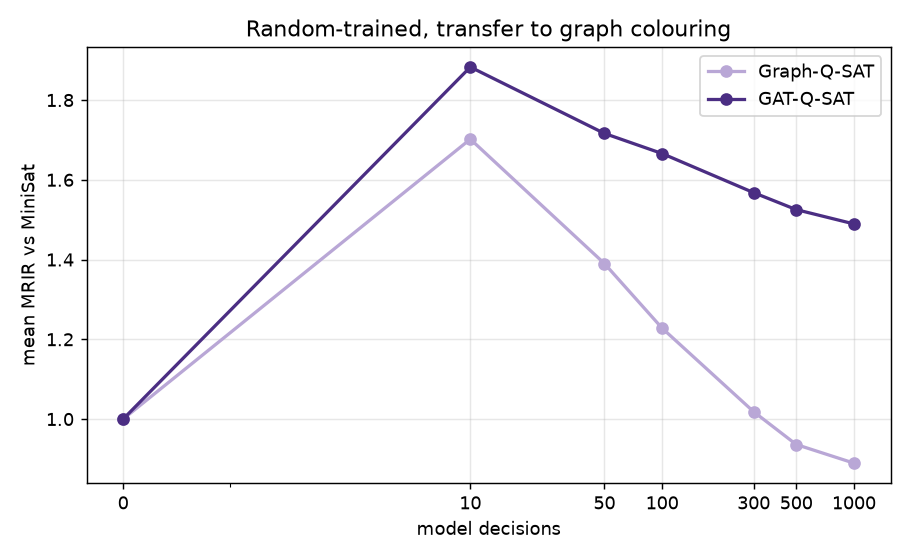
\includegraphics[width=0.62\textwidth]{random_transfer.png}
\caption{Random-trained models evaluated on graph colouring: MRIR against the
decision budget, averaged over the colouring families.}
\label{fig:transfercurve}
\end{figure}

\noindent
Figure~\ref{fig:gen} reads the same models across the size of the test
instances. The advantage of the attention model is stable and pronounced on
colouring at every size, while on random instances the ordering is reversed at
every size, so that neither effect is an artefact of one particular instance
set.

\begin{figure}[h]
\centering
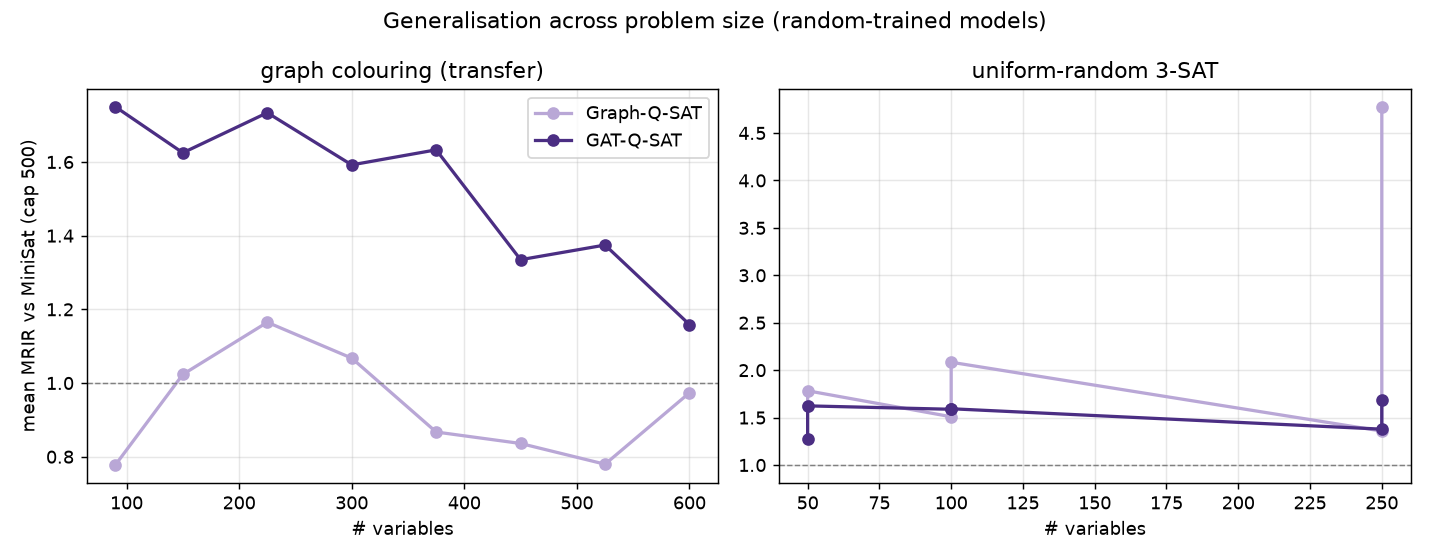
\includegraphics[width=0.88\textwidth]{generalization.png}
\caption{Random-trained models: MRIR against the number of variables of the test
instances (cap $500$).}
\label{fig:gen}
\end{figure}

\FloatBarrier
\subsection{A change of domain}\label{sec:transfer}

Uniform random 3-SAT has none of the structure of an application, so the rung
above answers an easier question than the one a user would ask, which is whether
a heuristic learned on the instances one happens to have is of any use on the
instances one actually cares about. We therefore take the colouring-trained
checkpoints of both models, with no retraining and no fine-tuning of any kind,
to four SATLIB families that they have never seen: small-world colouring (a
change of topology within the same problem), AIM (structured 3-SAT with a
controlled number of solutions), quasigroups (a combinatorial design problem)
and planning (the blocks-world and logistics encodings).
Figure~\ref{fig:transfer} gives the median MRIR at cap $200$.

\begin{figure}[h]
\centering
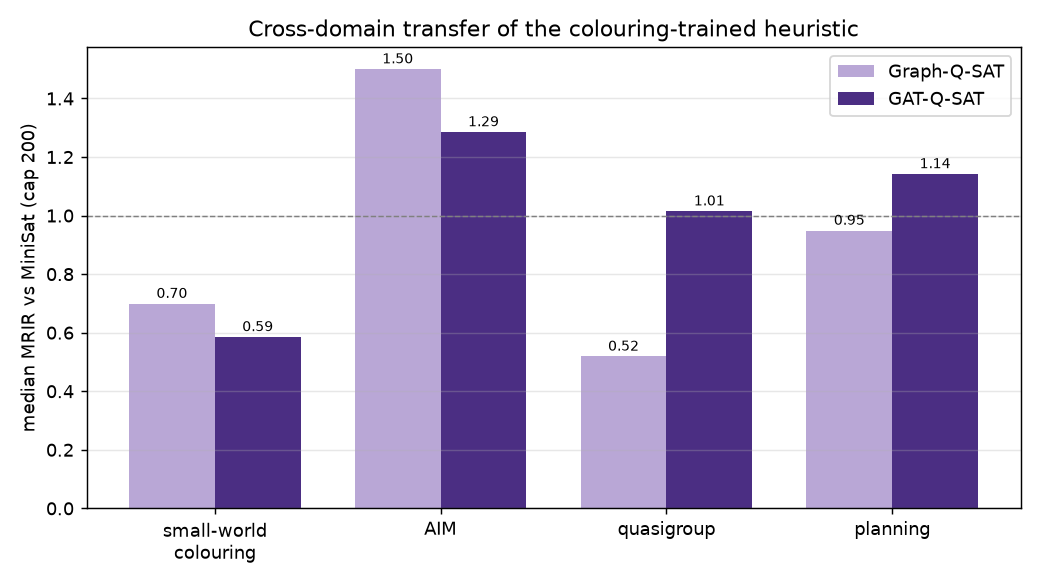
\includegraphics[width=0.70\textwidth]{transfer.png}
\caption{Transfer of the colouring-trained heuristic: median MRIR (cap $200$) on
four unseen SATLIB families.}
\label{fig:transfer}
\end{figure}

\noindent
GAT-Q-SAT is at or above the reference solver on three of the four families
(AIM $1.29$, quasigroup $1.01$, planning $1.14$) and Graph-Q-SAT on one of them
(AIM $1.50$). On the two families that have nothing to do with colouring
(quasigroups and planning) the attention model is above the solver and the plain
one below it. On AIM both transfer well, with the plain model marginally ahead;
on the small-world topology, which is the closest of the four to the training
problem, both fall below $1$. The last of these is worth a comment, since it is
the opposite of what one would guess: a change of topology within the same
problem hurts more than a change of problem. What the models carry across is
therefore not the problem they were trained on, but something coarser about the
shape of the graph, and it is precisely that coarser thing that the attention
coefficients appear to hold on to.

\smallskip
\noindent
It is worth noting that this is a preliminary study, and in which way. AIM (72
instances) and small-world (60) give medians one can rely on, but quasigroup
(11) and planning (8) are small families, so the numbers there are noisy; every
number is single-seed and at cap $200$. We had a reminder of what small samples
do here: the small-world median of Graph-Q-SAT was $2.42$ over 30 instances and
became $0.70$ over 60, i.e., the first figure was an artefact of the sample and
not a result. A larger panel, and more seeds, are what this measurement needs
before more weight is put on it.

\FloatBarrier
\subsection{The boundary, and a change of satisfiability}\label{sec:boundary}

Attention does not always help, and where it does not is as informative as the
rest. The models of this subsection are trained on satisfiable uniform random
formulas (\code{uf50-218} and \code{uf100-430}, two runs per variant), and
Figure~\ref{fig:randpair}
gives their MRIR family by family, on a common vertical scale. Graph-Q-SAT
reaches $4.78$ on \code{uf250-1065} at cap $500$ against the $1.69$ of
GAT-Q-SAT, i.e., a factor of three in favour of the plain aggregation on
instances five times larger than the training ones. This is the regime that
\S~\ref{sec:gat} predicts: a formula generated at the phase transition has, by
construction, no sub-structure that a weighting of the neighbours could exploit,
so the coefficients of \eqref{eq:gat} have nothing to learn, and the extra
parameters only make the fit harder.

\begin{figure}[h]
\centering
\begin{subfigure}{0.49\textwidth}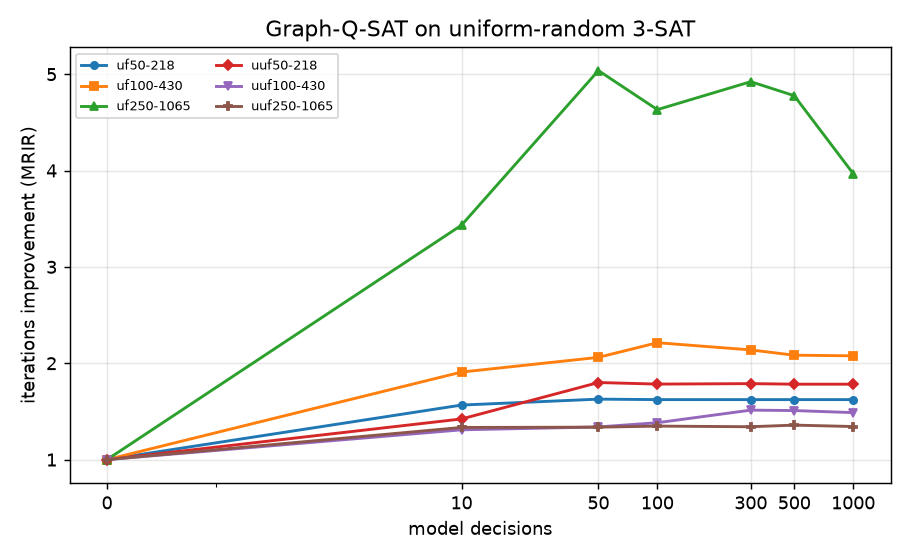
\includegraphics[width=\textwidth]{graphqsat_random.png}\end{subfigure}
\hfill
\begin{subfigure}{0.49\textwidth}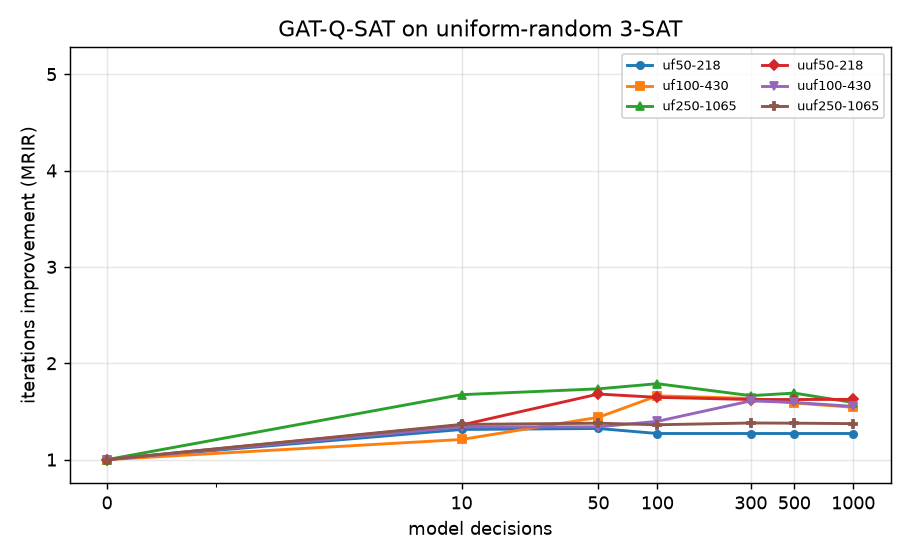
\includegraphics[width=\textwidth]{gatqsat_random.png}\end{subfigure}
\caption{Models trained on \code{uf50-218}: MRIR against the decision budget on
the satisfiable (\code{uf}) and unsatisfiable (\code{uuf}) random families, for
the plain model (left) and for the attention one (right), on a common vertical
scale. The whole advantage of the plain model lies in the \code{uf250-1065}
curve.}
\label{fig:randpair}
\end{figure}

\noindent
The same models give one further rung of the ladder for free. Having been trained
on satisfiable formulas only, they can be evaluated on the unsatisfiable families
of the same generator, where the search has to prove that no assignment exists
rather than to find one. Table~\ref{tab:unsat} reports the two sides at cap $500$:
the columns are the SATLIB families, the \code{uf} ones satisfiable and the
\code{uuf} ones unsatisfiable at the same size, and the rows the two models.

\begin{table}[h]\centering\small
\begin{tabular}{lccc@{\qquad}ccc}
\toprule
 & \multicolumn{3}{c}{satisfiable} & \multicolumn{3}{c}{unsatisfiable} \\
\cmidrule(r){2-4}\cmidrule(l){5-7}
 & \code{uf50-218} & \code{uf100-430} & \code{uf250-1065}
 & \code{uuf50-218} & \code{uuf100-430} & \code{uuf250-1065} \\
\midrule
Graph-Q-SAT & 1.62 & 2.08 & 4.78 & 1.61 & 1.45 & 1.21 \\
GAT-Q-SAT   & 1.27 & 1.59 & 1.69 & 1.62 & 1.69 & 1.45 \\
\bottomrule
\end{tabular}
\caption{Models trained on satisfiable random formulas (\code{uf50-218} and
\code{uf100-430}, mean over the two runs per variant), evaluated at cap $500$ on
the satisfiable and on the unsatisfiable families.}
\label{tab:unsat}
\end{table}

\noindent
The advantage of the plain aggregation does not survive the change of
satisfiability, and on the two larger families the ordering is reversed: where
the satisfiable side gives the plain model a gap of $3.09$ on
\code{uf250-1065}, the unsatisfiable one gives the attention model $1.69$
against $1.45$ at 100 variables and $1.45$ against $1.21$ at 250, the two being
level at 50. Two readings of this are possible, and the measurements do not
separate them: either the plain model has learned something about where the
satisfying assignments are, which is of no use when there are none, or proving
unsatisfiability leaves so little room to a branching heuristic that what
survives is the behaviour that transfers best anyway. The four runs trained
directly on the unsatisfiable families say that the regime is worth something to
the plain model and little to the attention one, since training on the target
takes Graph-Q-SAT from $1.61$ to $1.96$ on \code{uuf50-218} and GAT-Q-SAT from
$1.62$ to $1.63$. What can be said is that the regime in which the plain
aggregation wins is narrower than Figure~\ref{fig:thesis} alone suggests, and
that it is the one in which the question of \S~\ref{sec:transfer}, what survives
a change of the instances, has the least to do with structure.

\smallskip
\noindent
We remark that the plain model is very good here, and that this is the right way
to read the whole of \S~\ref{sec:results}: the question is not which of the two
models is better, but on which instances each of them is, and the answer is that
attention is the one that survives a change of the instances while the plain
aggregation is the one to use when there is nothing to weight.

\FloatBarrier
\subsection{Iterations against wall-clock time}\label{sec:time}

The MRIR rewards the reduction of the number of CDCL iterations, which is the
quantity the learned heuristic acts upon, and it is the metric of
\cite{Kurin2020}. Each decision, however, is a forward pass of the network, and
the attention of \eqref{eq:gat} makes that pass more expensive, so that a win in
iterations need not be a win in time. Figure~\ref{fig:time} reports the two
quantities side by side, per regime, at cap $500$. On colouring in distribution
GAT-Q-SAT takes the same time as Graph-Q-SAT ($1.1$ seconds) while performing
fewer iterations, so there the gain is real; on random 3-SAT it is about twice
as slow ($6.7$ seconds against $3.2$) and it also reduces the iterations less.

\begin{figure}[h]
\centering
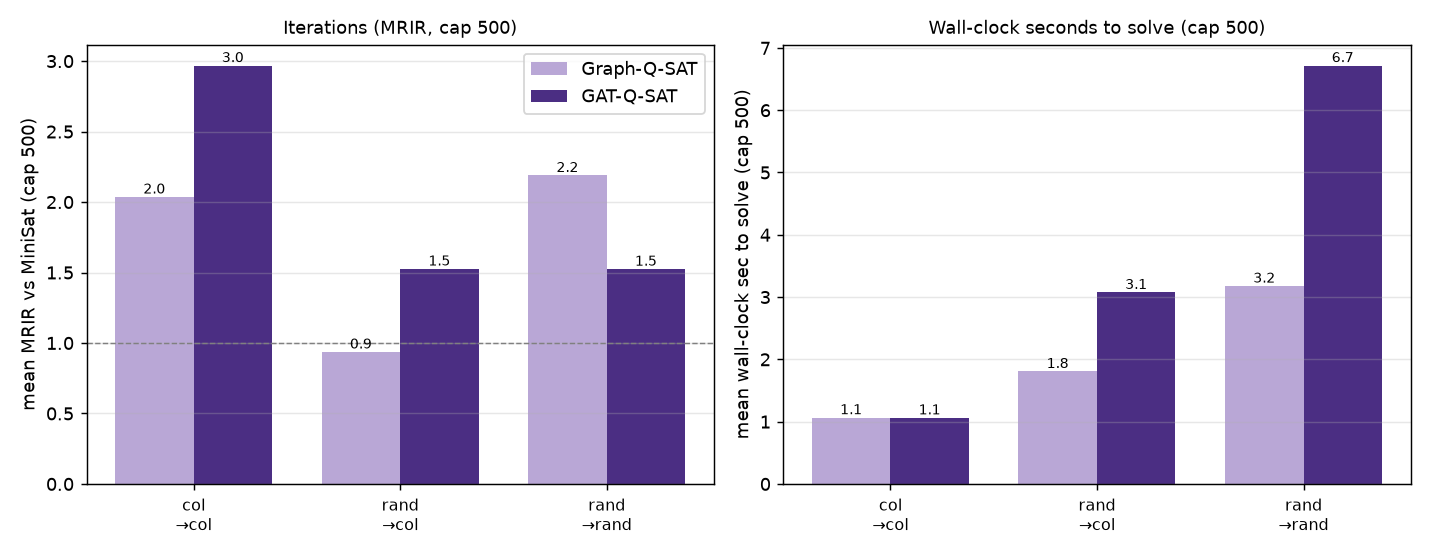
\includegraphics[width=0.92\textwidth]{mrir_time.png}
\caption{Iterations (left, MRIR) against wall-clock time (right, seconds to
solve), per regime, at cap $500$.}
\label{fig:time}
\end{figure}

\noindent
In absolute terms both agents take from $1$ to $7$ seconds on instances that
MiniSat solves in milliseconds, i.e., at this scale the per-decision cost of the
network dominates everything else, and the reduction of the iterations does not
become a speed-up. \smallskip
\noindent
The budget is where the two costs meet, and Table~\ref{tab:budget} reads them
together on the largest colouring family. The columns are three values of the
cap; for each model the table gives the mean wall-clock seconds to solve and the
mean MRIR at that cap. Going from cap $50$ to cap $1000$ costs Graph-Q-SAT
twenty-two times the time and takes its MRIR from $2.24$ to $0.98$, i.e., it
pays that time to end up slower than the solver it is guiding; GAT-Q-SAT pays a
factor of three and gains $0.11$, having reached at cap $50$ essentially all of
what it will ever reach. In both cases the decisions after the first fifty are
bought at full price and bring nothing, which is precisely the observation on
which the early release of \S~\ref{sec:impl} rests, and it is measurable on the
instances we have rather than on the large ones we do not.

\begin{table}[h]\centering\small
\begin{tabular}{lcc@{\qquad}cc@{\qquad}cc}
\toprule
 & \multicolumn{2}{c}{cap $50$} & \multicolumn{2}{c}{cap $500$} & \multicolumn{2}{c}{cap $1000$} \\
\cmidrule(r){2-3}\cmidrule(r){4-5}\cmidrule(l){6-7}
 & sec & MRIR & sec & MRIR & sec & MRIR \\
\midrule
Graph-Q-SAT & 0.48 & 2.24 & 5.14 & 1.35 & 10.71 & 0.98 \\
GAT-Q-SAT   & 1.13 & 3.28 & 3.90 & 3.39 &  3.80 & 3.39 \\
\bottomrule
\end{tabular}
\caption{Colouring-trained models on \code{flat200-479}: mean wall-clock seconds
to solve and mean MRIR, against the cap on the number of model decisions.}
\label{tab:budget}
\end{table}

\noindent
We state the absolute cost plainly because it is the one honest reading of these
instances: what is measured here is whether the learned heuristic makes
better decisions, not whether it makes them cheaply enough to be worth taking.
The restricted heuristics of \S~\ref{sec:impl} and the offline inference of
\cite{Wang2024} are the two answers the literature gives to this, and they are
answers to the same question, that of when the network is allowed to be queried.

%% ===========================================================================
\section{Conclusions}\label{sec:conc}
%% ===========================================================================

Replacing the uniform aggregation of a graph network with attention does not
make a learned branching heuristic much better on the instances it is trained
on: on the colouring family closest to the training one the two models are
within $0.17$ of MRIR of each other. What it changes is what the heuristic
carries with it when the instances change, and the four rungs of
\S~\ref{sec:results} measure exactly that. Across the size, the plain model
degrades to $1.35$ on instances four times larger than the training ones while
the attention one holds at $3.39$. Across the distribution, the plain model
falls below the heuristic it replaces at every size while the attention one
stays above it. Across the domain, with nothing retrained, the attention model
is at or above the reference solver on three families out of four and the plain
one on one. The advantage, in other words, grows with the distance between the
training and the test instances, which is the one reading that the three rungs
share, and it is a statement about transfer rather than about fit.

\smallskip
\noindent
The boundary is equally clear, and it is where the mechanism has nothing to work
on: on uniform random 3-SAT at the phase transition the neighbours of a node are
statistically alike, the coefficients of \eqref{eq:gat} have nothing to learn,
and the plain aggregation is better by a factor of three. That advantage, however, lives on the satisfiable instances alone: on the
unsatisfiable families of the same generator the attention model is ahead at 100
and at 250 variables and level at 50, so the regime in which the plain
aggregation wins is narrower than the aggregate figures suggest. A weighting of the neighbours, that
is, buys robustness to a change of the instances and pays for it where the
instances have no structure to be weighted; we would not know how
to choose between the two models without knowing which of the two situations one
is in.

\smallskip
\noindent
The list of what is missing is short, and none of it is hidden in the numbers
above. The transfer study rests on two families of 72 and 60 instances and on
two of 11 and 8, single-seed and at one cap, which is enough to see an effect of
that size but not to put an error bar on it. The small-world family, where both
models fail, is the one that a larger panel should explain first, since it is
the family closest to the training problem and the one on which the models do
worst; a reading in terms of the degree distribution of the graph, rather than
of the problem that generated it, is what we would look for there. The
wall-clock cost of a decision is not addressed at all here: the restricted
heuristics are implemented, but measured only on instances too small for them to
pay. The natural next step is to run them where the solve is heavy enough to
dominate the inference, which is also where the offline, one-shot inference of
\cite{Wang2024} would have to be compared against them. Finally, the whole study
is built on one architecture and one metric. The benchmark of \cite{Li2023} and
the analysis of \cite{Mojzisek2025} exist to say how much of a result of this
kind is a property of the method rather than of the design choices around it,
and we have not used them.

%% ===========================================================================
\section*{Acknowledgements}\label{sec:ack}
%% ===========================================================================

The implementation that we started from is the one of Kurin et al.
\cite{Kurin2020}, released with the paper, and the solver underneath it is
MiniSat \cite{EenSorensson2003}.

%% ===========================================================================
\bibliographystyle{plain}
\bibliography{gatqsat}

%% ===========================================================================
\appendix
\section{The instances, and how the numbers are regenerated}\label{app:instances}
%% ===========================================================================

Every instance used here comes from SATLIB \cite{HoosStutzle2000}, in DIMACS
form, and is stored in the repository so that no download is needed. The
uniform random 3-SAT families are \code{uf50-218} and \code{uuf50-218},
\code{uf100-430} and \code{uuf100-430}, \code{uf250-1065} and
\code{uuf250-1065}, the satisfiable and unsatisfiable formulas at the phase
transition; the graph-colouring ones are \code{flat30-60}, \code{flat75-180},
\code{flat125-301}, \code{flat150-360} and \code{flat200-479}, the name giving
the number of nodes and of edges of the graph to be 3-coloured. Training uses
\code{flat50-115} for the colouring-trained models and the random families for
the others, with the usual split into training, validation and test parts; the
evaluations of \S~\ref{sec:results} are run on the test parts only.

\smallskip
\noindent
The four families of \S~\ref{sec:transfer} are the small-world colouring set
(60 instances, 500 variables and 3100 clauses each, obtained by 5-colouring
small-world graphs on 100 vertices, the family index moving the graph from a
ring lattice to a random one), AIM (72 instances of structured 3-SAT with a
controlled number of solutions), quasigroups (11 instances, up to 729
variables) and planning (8 instances from the blocks-world and logistics
encodings, up to 1200 variables). None of them is used for training, in any
form.

\smallskip
\noindent
Before a family can be evaluated, the reference iteration counts that
\eqref{eq:mrir} divides by are computed once and stored next to it, so that the
baseline is fixed and the same for every model. The evaluation of one
checkpoint on one family at one cap writes one line per instance, with the
wall-clock time, the episode and the ratio; the tables and the figures of \S~\ref{sec:results} are produced from those lines by four scripts, one that aggregates the runs into a summary, one that draws the curves, one that groups the runs by attention and by training set to produce the ablation, and one that runs and draws the transfer study. The last two write their figures next to this note when the output directory is set to \code{report/img}, which is where the ones printed here come from. There is no manual step in between, and no spreadsheet: every number in this note is regenerated by running those scripts on the committed logs.

\end{document}
